\chapter{Wo steckt die zweite L"osung?\label{chapter:thema}}
\lhead{Bessel-Funktionen zweiter Art}
\begin{refsection}
\chapterauthor{Stefan Kull und Roy Seitz}

\newcommand*\sk{\vcenter{\hbox{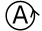
\includegraphics[scale=0.4]{komplex/SK_operator.pdf}}}}

\printbibliography[heading=subbibliography]
\end{refsection}

